\section{Описание методов и инструментов для реализации}

\subsection{Система для промышленного интернета вещей}

Как было описано в предыдущей главе,
промышленный анализ данных предоставляет идеи для создания
интеллектуальной системы для автоматизации и повышения
эффективности работы промышленных устройств.
Одной из множества компаний, которая ведет деятельность в данной области,
является компания Omnicube.

Компания Omnicube разарабатывает и предоставляет универсальную платформы
для решения различных задача интеллектуального мониторинга
на предприятиях различных отраслей: промышленность,
интеллектуальные сервисы для зданий, мониторинг персонала,
экологический мониторинг, сервисы для предприятий сельского хозяйства,
инструменты для медицинских учреждений. \cite{omnicube}

\begin{figure}[h]
    \center{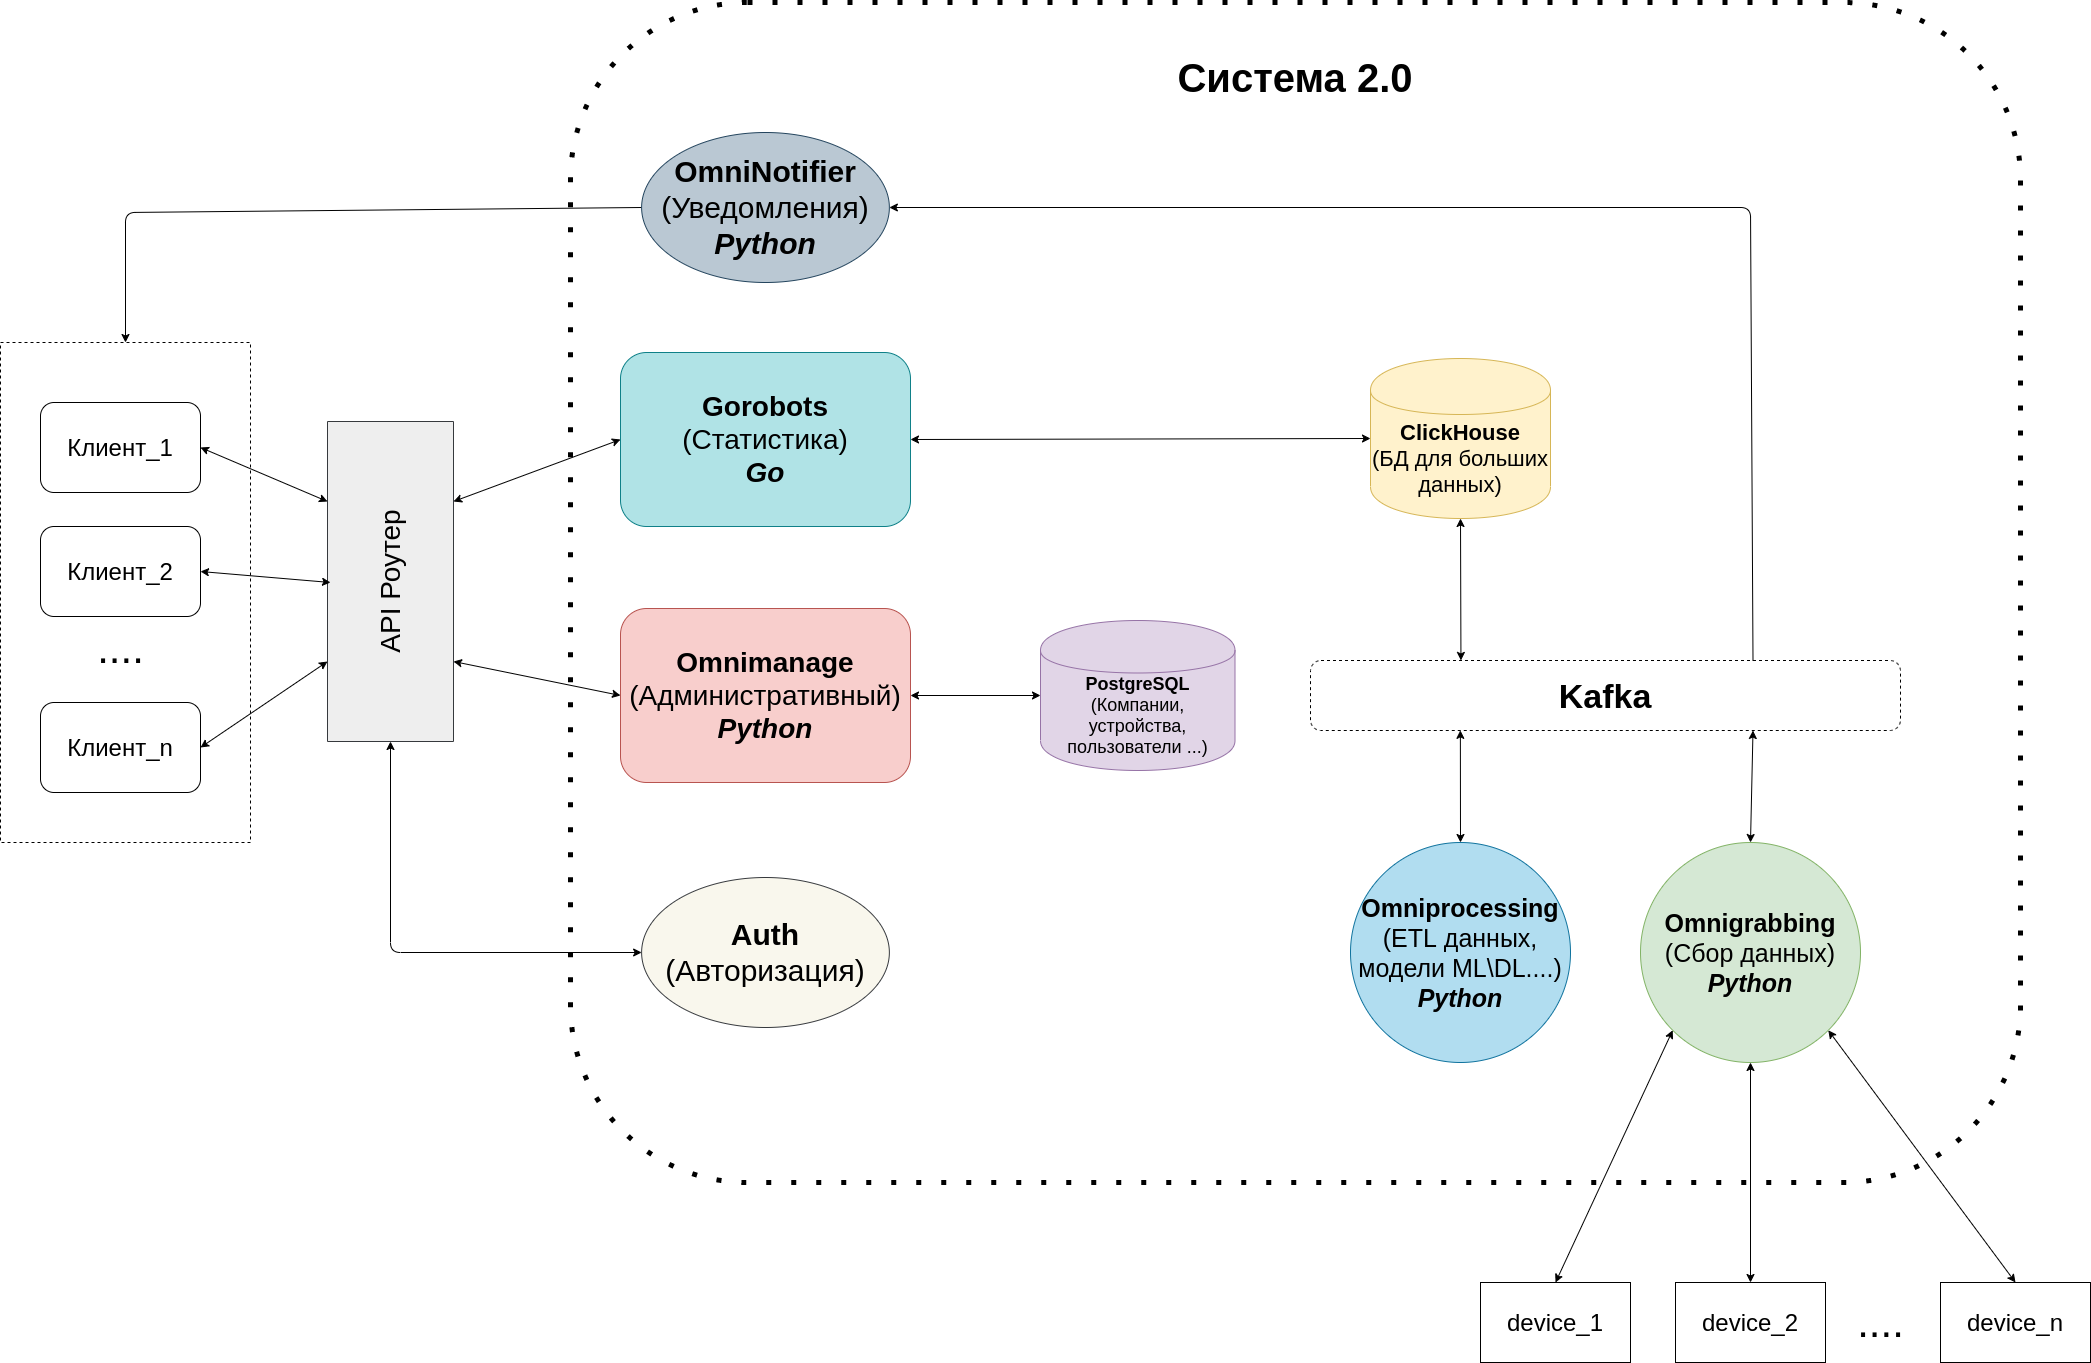
\includegraphics[width=15cm]{img/sys2.png}}
    \caption{Разработанная система для интернета вещей}
\end{figure}

Данная система имеет микросервисную архитектуру.
У каждого микросервиса существует своя совокупность задач,
которую он решает. Опишем основные принципы работы микросервисов.

Микросервис omniprocessing является местом, где располагаются различные модели для мониторинга и обработки данных,
например, модели машинного обучения.
Основные цели данного микросервиса -- извлечение, трансформация и загрузка.

В omniprocessing используется Python фреймфорк Faust, который позволяет отправлять
данные в очередь брокеру сообщений Kafka. Из Kafka данные попадают в базу данных ClickHouse.
Благодаря данному фреймворку можно быстро строить и встраивать пайплайны машинного обучения. \cite{faust}

(Kafka: описание и обонование использования)

(ClickHouse: описание и обоснование выбора)

(Faust: описание фреймворка и обоснование выбора)

(Место модели в микросервисе)

(выбрали вот такой способ обучения и обновления в реальном времени)

\subsection{Модель выявления признаков}

(описания метода кластеризации t-Shape)

(градиентный бустинг)

(описание обучения в реальном времени со скользящим окном)

\subsection{Модель предсказания}

\subsection{Выводы}

\clearpage